% Ancestry of one myth: Agent 1's round-4 myth in the September Sonnet 4.5
% population run rep00 (negative_only_reasoning_rerun_population_myth_game_claude_n5,
% noisy8_crossmodel_negative_twotask_r3). Each myth has two inputs: the writer's own
% previous myth (chat memory) and the myth shown in the prompt (previous round's
% partner's myth). Pairings from the run's conversation_history.
\documentclass[tikz,border=8pt]{standalone}
\usepackage[T1]{fontenc}
\usepackage{lmodern}
\renewcommand{\familydefault}{\sfdefault}
\usetikzlibrary{arrows.meta}
\begin{document}
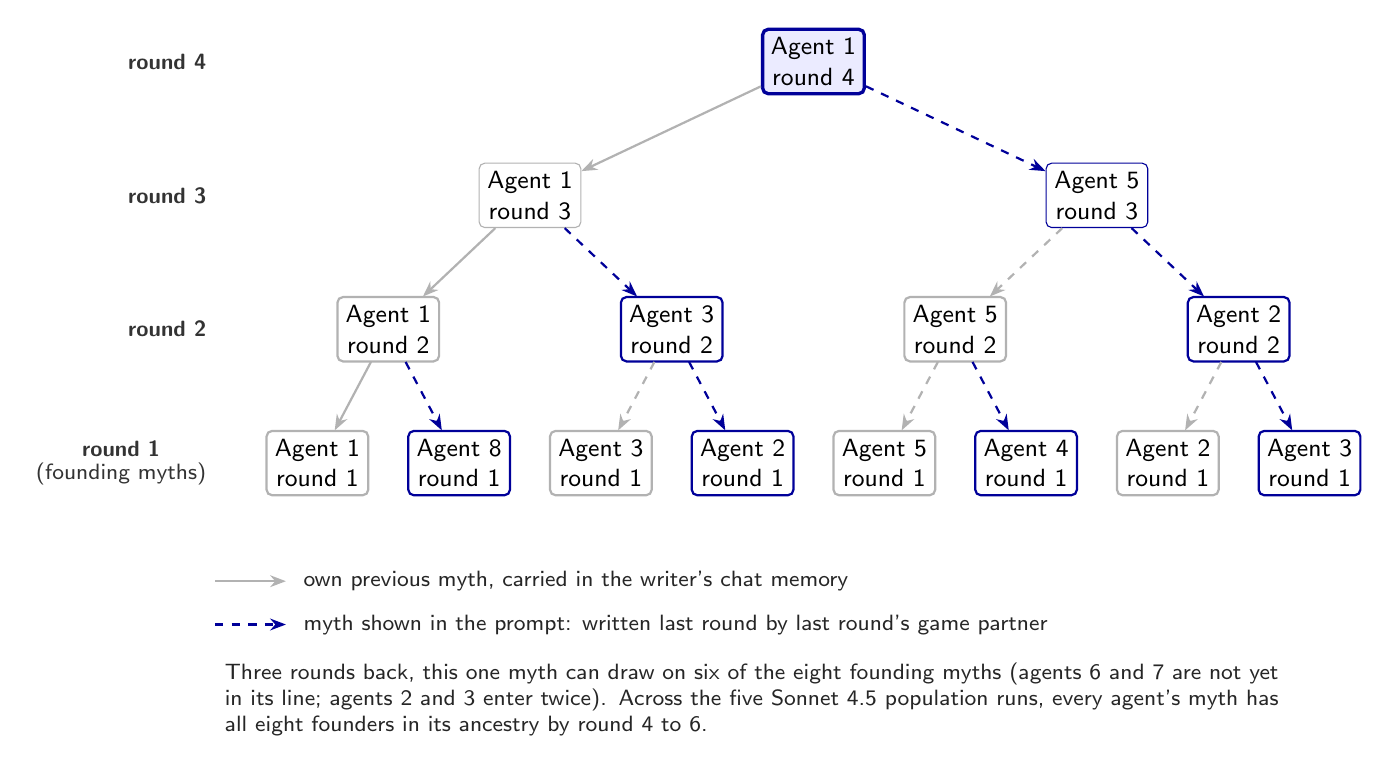
\begin{tikzpicture}[
  font=\small,
  grow=down,
  level distance=17mm,
  level 1/.style={sibling distance=72mm},
  level 2/.style={sibling distance=36mm},
  level 3/.style={sibling distance=18mm},
  every node/.style={draw, rounded corners=2pt, align=center, inner sep=3pt, fill=white},
  root/.style={draw=blue!60!black, solid, very thick, fill=blue!8},
  own/.style={draw=gray!60, solid},
  shown/.style={draw=blue!60!black, solid},
  edge from parent/.style={draw, thick, gray!60, ->, >={Stealth[length=2mm]}},
  ownedge/.style={edge from parent/.style={draw, thick, gray!60, ->, >={Stealth[length=2mm]}}},
  shownedge/.style={edge from parent/.style={draw, thick, blue!60!black, dashed, ->, >={Stealth[length=2mm]}}},
  rnd/.style={draw=none, fill=none, font=\footnotesize\bfseries, text=gray!40!black, anchor=east},
]
\node[root] {Agent 1\\round 4}
  child[ownedge]   {node[own] {Agent 1\\round 3}
     child[ownedge]   {node[own]   {Agent 1\\round 2}
        child[ownedge]   {node[own]   {Agent 1\\round 1}}
        child[shownedge] {node[shown] {Agent 8\\round 1}}}
     child[shownedge] {node[shown] {Agent 3\\round 2}
        child[ownedge]   {node[own]   {Agent 3\\round 1}}
        child[shownedge] {node[shown] {Agent 2\\round 1}}}}
  child[shownedge] {node[shown] {Agent 5\\round 3}
     child[ownedge]   {node[own]   {Agent 5\\round 2}
        child[ownedge]   {node[own]   {Agent 5\\round 1}}
        child[shownedge] {node[shown] {Agent 4\\round 1}}}
     child[shownedge] {node[shown] {Agent 2\\round 2}
        child[ownedge]   {node[own]   {Agent 2\\round 1}}
        child[shownedge] {node[shown] {Agent 3\\round 1}}}};
% round labels on the left
\node[rnd] at (-7.6,0)    {round 4};
\node[rnd] at (-7.6,-1.7) {round 3};
\node[rnd] at (-7.6,-3.4) {round 2};
\node[rnd] at (-7.6,-5.1) {round 1\\[-1pt]\mdseries(founding myths)};
% legend + reading
\begin{scope}[every node/.style={draw=none, fill=none, align=left, anchor=west, font=\footnotesize, text=gray!30!black}]
  \draw[thick, gray!60, ->, >={Stealth[length=2mm]}] (-7.6,-6.6) -- (-6.7,-6.6);
  \node at (-6.6,-6.6) {own previous myth, carried in the writer's chat memory};
  \draw[thick, blue!60!black, dashed, ->, >={Stealth[length=2mm]}] (-7.6,-7.15) -- (-6.7,-7.15);
  \node at (-6.6,-7.15) {myth shown in the prompt: written last round by last round's game partner};
  \node[text width=13.4cm] at (-7.6,-8.1) {Three rounds back, this one myth can draw on six of the eight founding myths (agents 6 and 7 are not yet in its line; agents 2 and 3 enter twice). Across the five Sonnet 4.5 population runs, every agent's myth has all eight founders in its ancestry by round 4 to 6.};
\end{scope}
\end{tikzpicture}
\end{document}
